\def\PicPath{/Users/ken/Documents/shuron/chapter1/1_2}

\begin{comment}

(図\ref{fig:science_sensitivity})
\begin{figure}
\centering
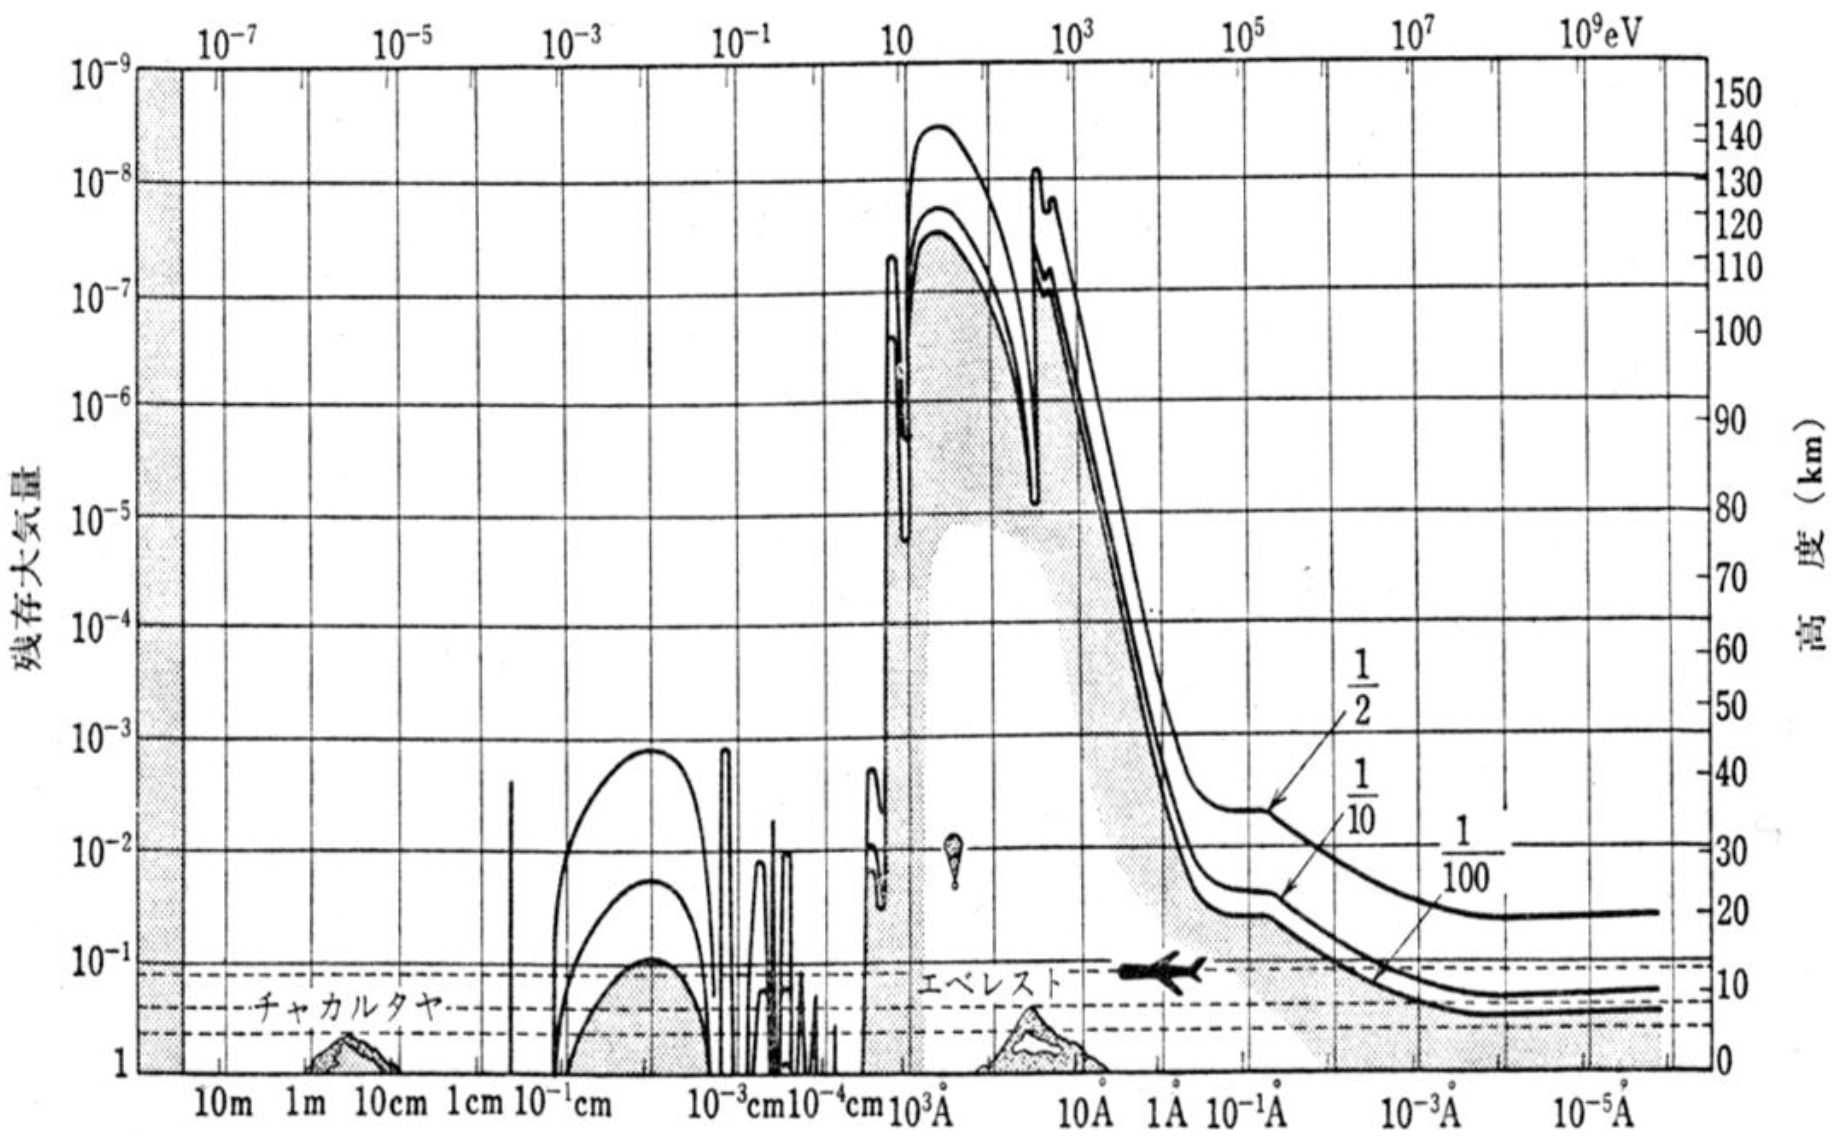
\includegraphics[width=15cm]{\PicPath/atmosphere_absorption.png}
\caption{大気による様々な波長の電磁波の吸収(出典??)\cite{oda_and_matsuoka}}
\label{fig:atm_absp}
\end{figure}

\end{comment}

\section{核ガンマ線観測}
核ガンマ線の観測をするとめっちゃうれしいよ!こういうことがわかるしなんでもわかる
\subsection{核ガンマ線}
てすとてすと
\subsection{Ia}
テストテスト
\subsection{重力崩壊型}
テストテスト



